%
%

%%-----------------------------------------------------
%%-----------------------------------------------------
\section{Texto para todos los gustos}

%%-----------------------------------------------------
\begin{frame}
\frametitle{Unicode}

\begin{columns}[T]
\begin{column}{.48\textwidth}

\includegraphics[width=5cm]{figs/unicode-logo}

\vspace{.5cm}

{\Large

\begin{flushright}
\url{http://unicode.org/}
\end{flushright}
}

\end{column}%
\hfill%
\begin{column}{.60\textwidth}
  {\Large
    Meta: texto en cualquier sistema de escritura
    
    \begin{itemize}
    \item codificación
    \item representación
    \end{itemize}

    \vspace{.2cm}
    
    \begin{itemize}
    \item 129 sistemas de escritura
    \item conjuntos de otros símbolos
    \item más de 120.000 caracteres
    \end{itemize}
  }
\end{column}%
\end{columns}

\end{frame}

%%-----------------------------------------------------
\begin{frame}
\frametitle{Principios}

{\Large
\begin{itemize}
\item Se codifican los grafemas (definición abstracta)
\item No trata sobre la representación
\item Cada grafema, un número (31 bits) \\
  Ejemplo: U+00F1 (ñ) \\
\item U+0000 -- U+00FF: Latin-1
\end{itemize}

\vspace{.2cm}

Codificaciones:

\begin{itemize}
\item UTF-8: anchura variable, compatible con ASCII
\item UTF-16: anchura variable, mejor para ideogramas
\item UTF-32: anchura fija
\end{itemize}
}

\end{frame}

%%-----------------------------------------------------
\begin{frame}
\frametitle{Primeros caracteres}

\begin{center}
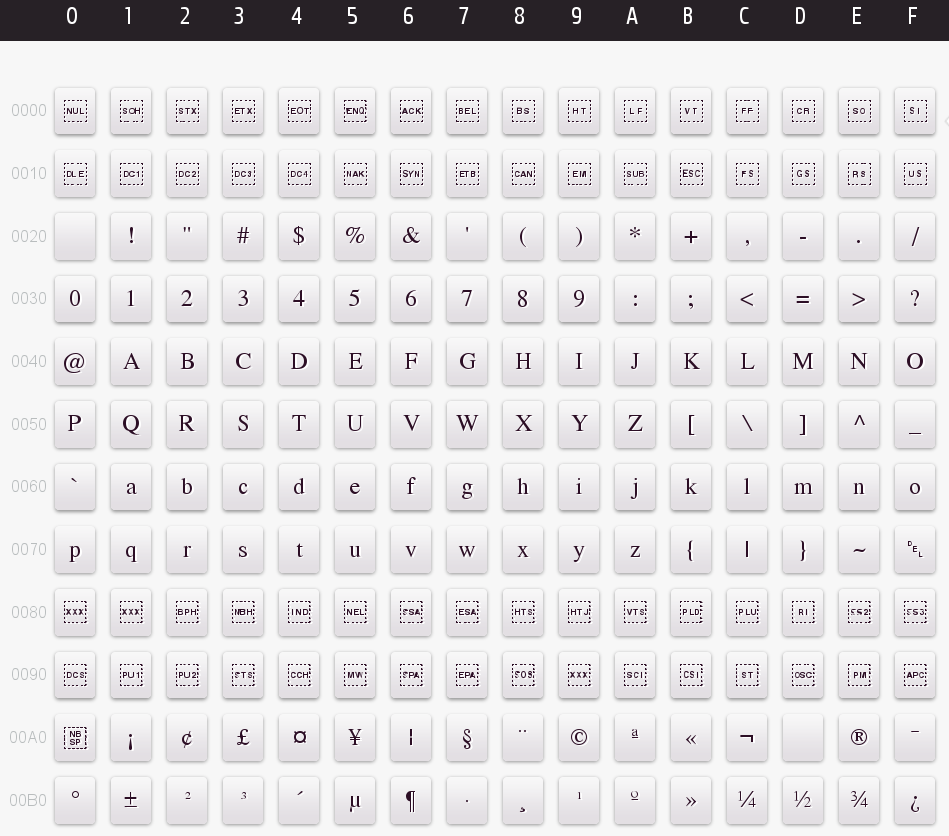
\includegraphics[width=9cm]{figs/unicode-0000}
\end{center}

\end{frame}

%%-----------------------------------------------------
\begin{frame}
\frametitle{Caracteres arábicos}

\begin{center}
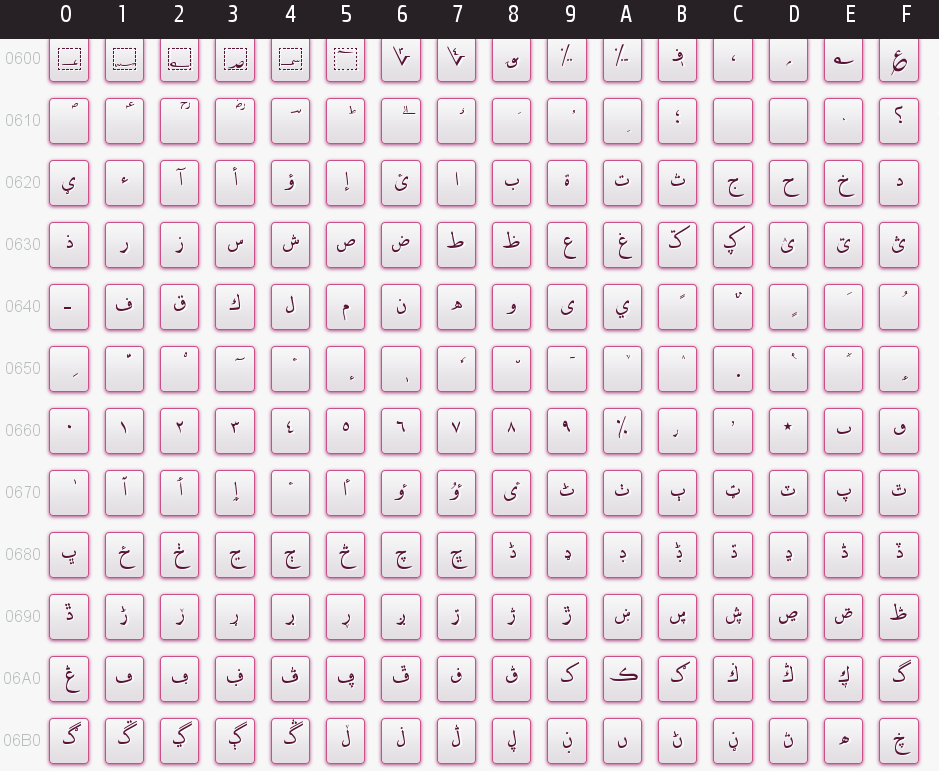
\includegraphics[width=9cm]{figs/unicode-0600}
\end{center}

\end{frame}

%%-----------------------------------------------------
\begin{frame}
\frametitle{Emojis}

\begin{center}
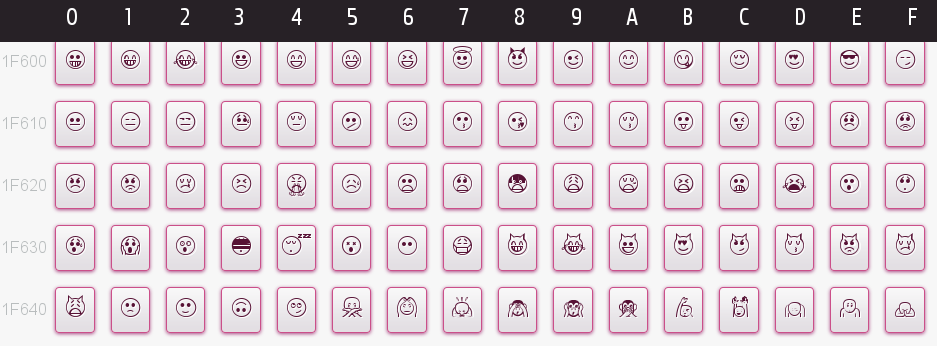
\includegraphics[width=9cm]{figs/unicode-emoji}
\end{center}
\end{frame}

%%-----------------------------------------------------
\begin{frame}

\begin{center}
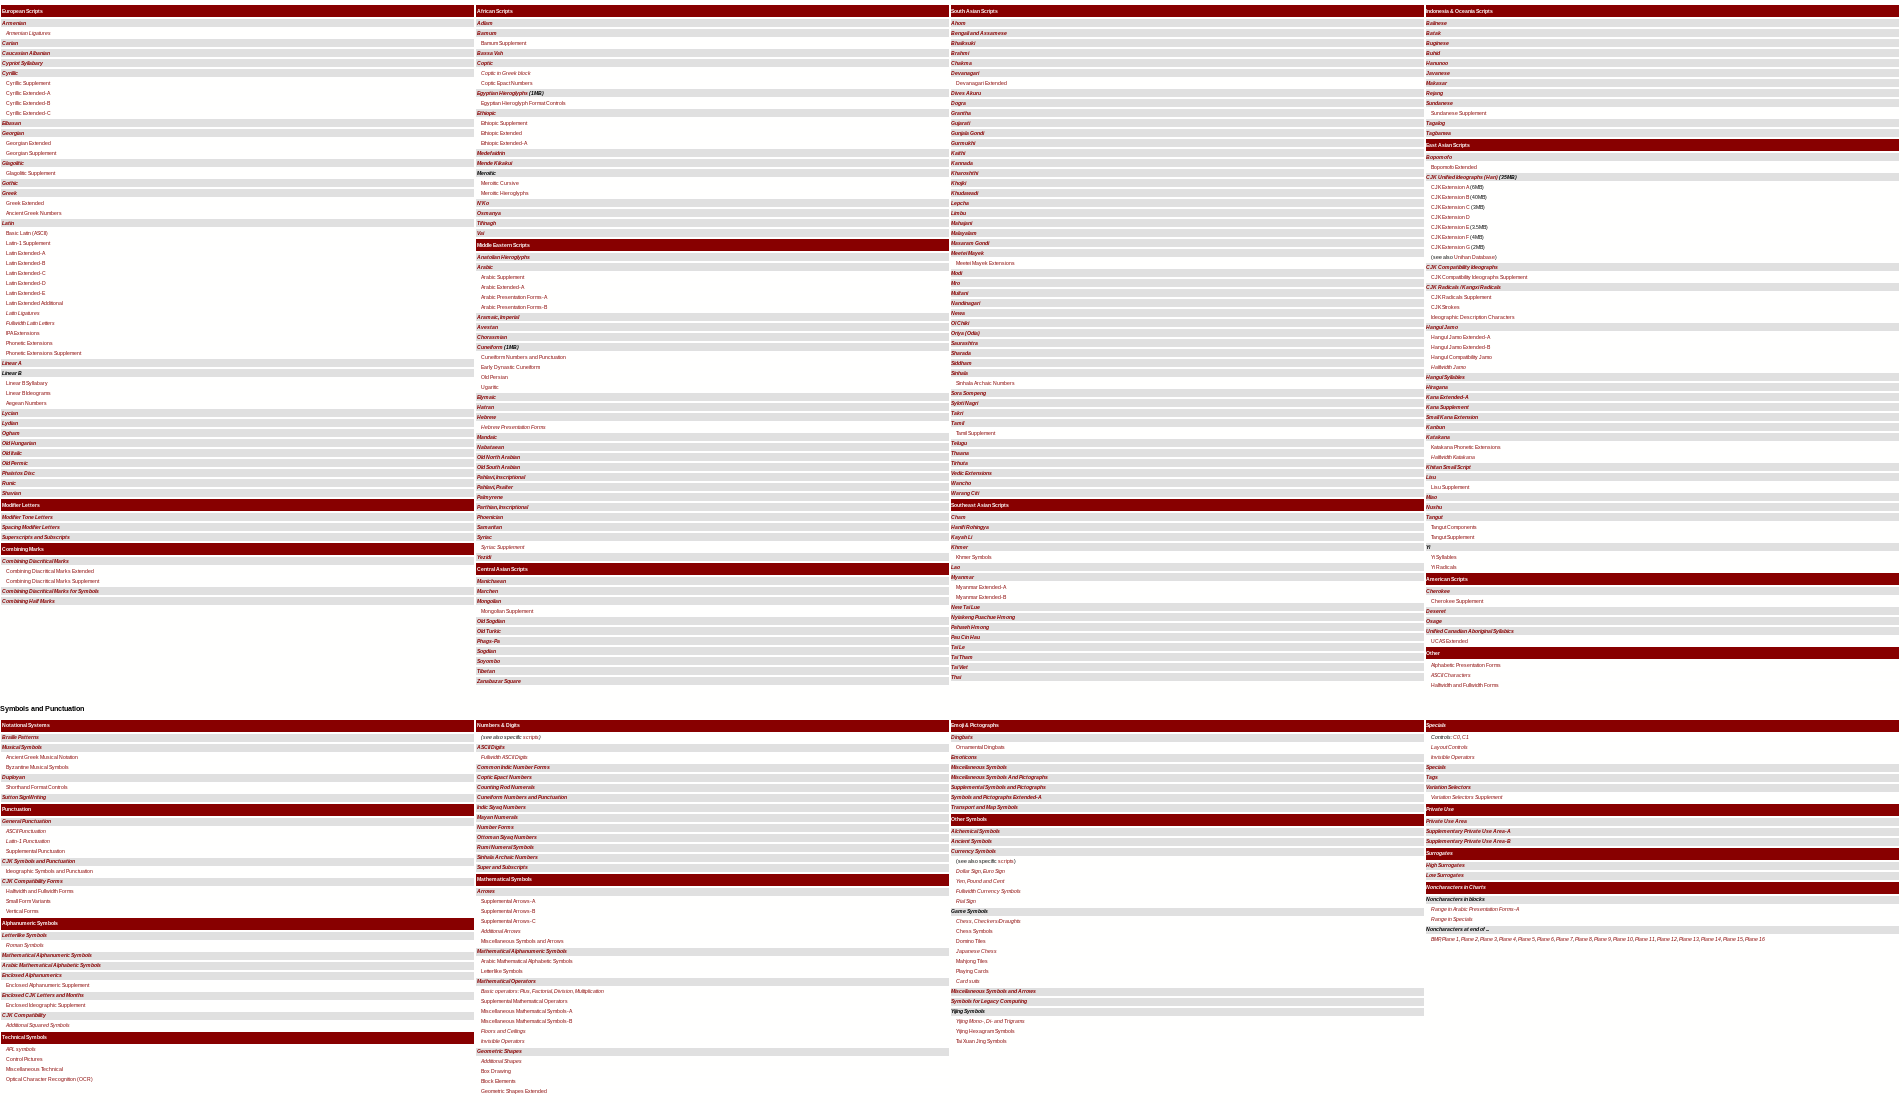
\includegraphics[width=11cm]{figs/unicode-charts}
\end{center}

\begin{flushright}
\url{http://www.unicode.org/charts/}
\end{flushright}
\end{frame}

